% This is LLNCS.DOC the documentation file of
% the LaTeX2e class from Springer-Verlag
% for Lecture Notes in Computer Science, version 2.4
\documentclass{llncs}
\usepackage{llncsdoc}
\usepackage[T1]{fontenc}
\usepackage[utf8]{inputenc}
\usepackage{graphicx}
\graphicspath{{Images/}}
%
\begin{document}
    \title{Context Aware Virtual Assistant with
    Case-Based Conflict Resolution in
    Multi-User Smart Home Environment}
    \author{Bauyrzhan Ospan\inst{1} \and Nawaz Khan \inst{2} \and Juan Augusto \inst{2} \and Mario Quinde \inst{2} \inst{3} \and Kenzhegali Nurgaliyev \inst{1}}
    \institute{Department of Information Technology, Kazakh University of Technology and Business, Kayim Muhamedhanov 37A, Astana 010000, Kazakhstan \\ \email{{bospan,knurgaliev}@nu.edu.kz}
    \and Department of Computer Science, Middlesex University, The Burroughs, London NW4 4BT, United Kingdom \\ \email{{N.X.Khan,J.Augusto,MQ093}@live.mdx.ac.uk}
    \and Department of Industrial and Systems Engineering, Universidad de Piura, Av. Ramon Mujica 131, Urb. San Eduardo, Piura, Peru\\
    \email{mario.quinde@udep.pe}}
    \maketitle
    \begin{abstract}
        In this work we will examine and develop a Virtual Assistant that is used as a control
        interface of the Smart Home environment in the Farm Side Middlesex University laboratory.
        Specifically, the system is
        constructed to give multiple users ability to control devices by voice or text commands through the dialogue
        interface.
        The main purpose of the research is to create user friendly interface with adaptive context aware
        Case-Based conflict resolution system.
        In addition, Feed-Forward Artificial Neural Networks were used to classify user inputs, voice
        recognition and voice generation instruments were used to implement natural dialogue model of interactions with users.
        Further, a set of randomised double-blinded
        evaluation tests were established.
    \end{abstract}
    \begin{keywords}
        Case-Based Reasoning, Context Awareness, Multiple User systems, Smart Home, Virtual Assistant
    \end{keywords}
    %
    \section{Introduction}
    %
    Managing a comfortable Activities of Daily Life (ADL) could be a challenging task for people with special needs
    and younger population \cite{9}.
    As a result,
    the Smart Home environments are developed to help users in controlling devices \cite{13}
    that are often called Virtual Assistants \cite{9} or monitor behaviours of people
    with special needs \cite{3} to classify changes in ADL that then alarm or notify relatives, health and care professionals
    and organizations \cite{15}.
    Additional finding identified other techniques in the state of art.
    For example, in Smart Home systems there are Ontology-based platforms that allows to analyze user`s actions and
    perform context recognition \cite{1} or visual tools for creating personal preferences table of each user based on semantics
    metadata \cite{8}.
    As a consequence, majority of the researches is aimed to develop systems that helps alone living users.\\
    On the other hand, conflicting orders inside the system by different users can lead to the risks \cite{5}.
    Despite number of
    researches in the Smart Home solutions that are automated, adaptive, multifunctional and interactive, there is a lack of
    investigations and development of systems that operates in a conflict resolution between multiple users with different
    needs and priorities.
    Some researchers in order to solve this dilemma developed context-aware automation platforms
    \cite{5,6} that resolves conflicts between automated devices.
    These solutions resolves conflicts only between automated devices based on priorities.
    The next group of
    developers are focused on preference Rule-Based Reasoning (RBR) \cite{9}.
    Even through
    these systems introduce efficient set of rules, they are not able to handle with adaptation. \\
    In this research, we propose a Virtual Assistant (VA) system that controls Smart Home environment based on the user inputs via
    voice and text based dialogue graphical web user interface for multiple users and resolve conflicts in changing environment.
    The architecture of the system is
    described in the Section II. The system algorithms and sequences are described in the Section III. Section IV demonstrates
    our results and validation.
    Finally, Section V draws the conclusion and predictions for the future work.
    %
    \section{Architecture}
    %
    Technical details of the system
    consider architecture diagram of the system and explanation of all functional units called modules
    or divided into the groups called components.
    We have used updated user types and preference system proposed by \cite{9}.
    Moreover, argument priorities were established by personal user preferences \cite{11} because
    number of researches shows that the preference-based argumentation increases ability of the systems to meet user
    expectations \cite{10}.\\
    The preferences are reasons why user wants to change the device status.
    Introducing reason is the way to increase usability of the system through the implicit interpretation of user needs.
    Context awareness of the system is the key for creating high usability via making the interaction
    between user and system more natural \cite{7}.
    We have used "Ceteris paribus" preferences binary tree representation.
    At the moment, CP-nets are most effective qualitative approach for presenting preferences in the strict known
    environment as the Smart Home \cite{10}.\\
    \begin{table}
        \caption{List of users and preferences}
        \begin{tabular}{llllll}
            \hline\noalign{\smallskip}
            User types & Preferences (positions 0,1,2,3,4,5)\\
            \noalign{\smallskip}
            \hline
            \noalign{\smallskip}
            Adult (26-69 ages) & Security, Health, Work, Food, Energy, Entertainment\\
            Elderly (older 70) & Health, Security, Food, Energy, Entertainment, Work\\
            Young (up to 25 ages) & Security, Work, Entertainment, Health, Food, Energy\\
            \hline
        \end{tabular}
    \end{table}
    The architecture of the system is layered and modular.
    As a result, each functional part (module) of the system is designed to execute complete task.
    The component is group of modules that performs complex task that consists of a number of simple tasks.
    For example, Order Classification and Reason Classification modules are grouped to Classification component.\\
    In addition, in order to give better understanding of the system, the architecture is divided into layers.
    Layer is functional level of the system that sequentially divides it into hierarchical groups that
    communicates only with layer above or layer below except Database layer.\\
    Layer is demonstrated as white rectangle with grey icon and name in it.
    Web pages of the web interface is demonstrated as white colored box with blue drawing and text in it.
    Blue hexagonal icon with white image inside and text below is module of the system.
    White quadrilateral with grey illustration of device and it`s name underneath is icon of electronic device driven
    by Smart Home environment.
    Colored rectangle with text in the bottom right corner is illustration of components.
    All communications inside the system is demonstrated as arrows in the Fig.1.
    \footnote{Communication types and lifelines of the system is described in the Section III.}
    \begin{figure}
        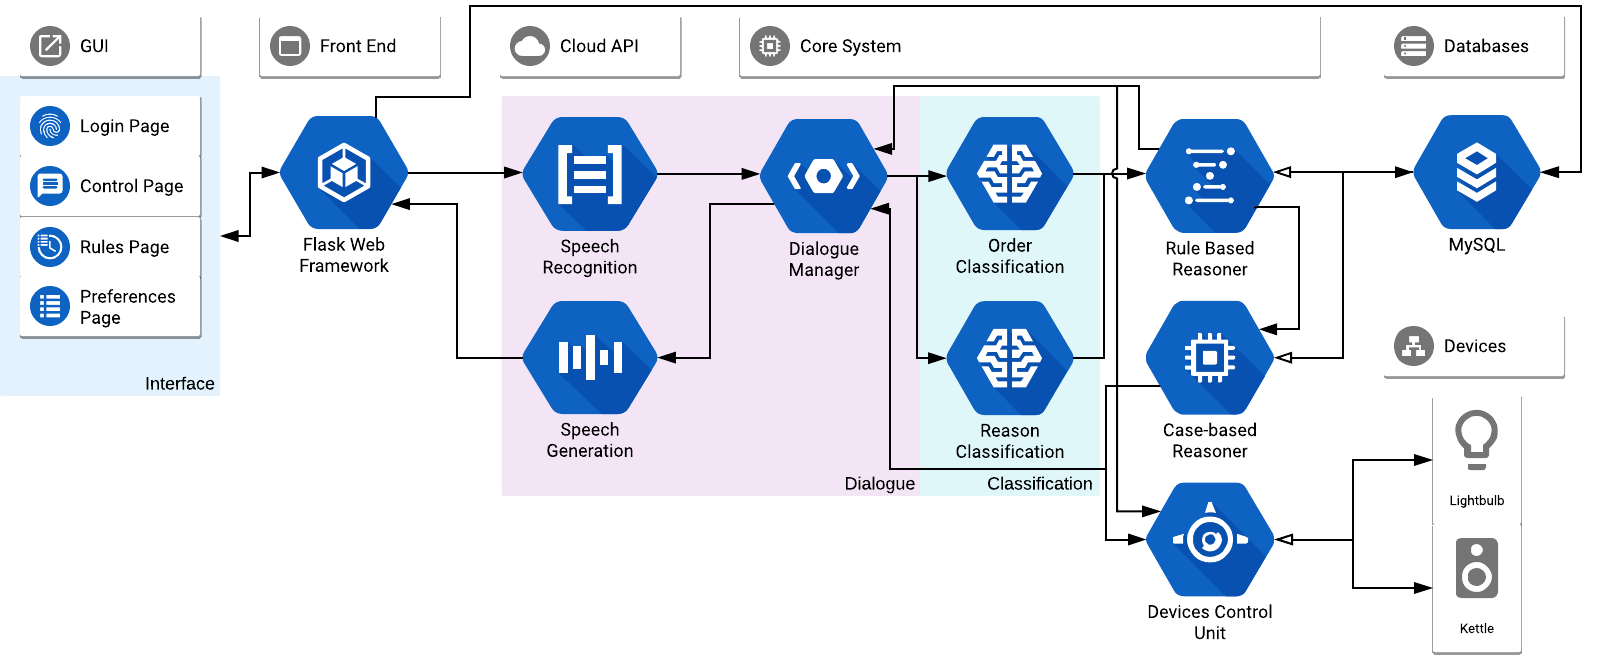
\includegraphics[width=\textwidth]{arch.png}
        \caption[]{Architecture diagram of the system}
    \end{figure}
    \subsection{Graphical User Interface, Front End and Cloud API}
    The interface of the system is graphical web interface developed as web site shown in the figure below.
    Graphical User Interface (GUI) is expressed by 3 functional and one login pages.\\
    \begin{figure}
        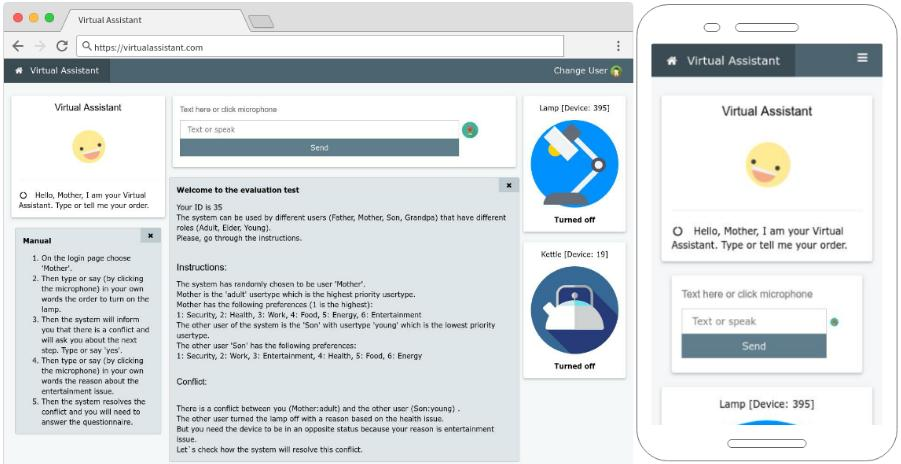
\includegraphics[width=\textwidth]{mockup.png}
        \caption[]{Control Page of the web interface}
    \end{figure}
    Firstly, header menu with hyperlinks to each page is located on the top of the interface.
    In the upper left corner of the Control Page there are emotional icon representing facial expressions of the Virtual Assistant
    and text of the VA answers below it.
    In addition, usage manual is provided below VA that can be easily closed by clicking "x" button.
    In the middle of the page, you can find input box with microphone activating and send buttons.
    In order to explain system, there is instruction block under the input box.
    Last but not the least, right hand side of the interface is filled by devices status indicators that shows current statuses.\\
    The function units of the Speech Generation and Speech Recognition were established via W3C Web Speech API.
    They are JavaScript Application Programming Interfaces (API) that are used by most of the modern browsers.
    As a result, the system sends record of the user input to W3C API and it returns recognised text.
    Moreover, the system sends text to the browser of the user in such way that the browser automatically generates it into voice.
    \subsection{Core System}
    Core System is main functional layer.
    Consequently, functions as decision-making, dialogue compilation, text classification and device controlling are all executed in the Core System.
    It consists of Dialogue Manager, Classification Component, Rule-Based Reasoner, Case-Based Reasoner and Device Control Unit.\\
    Classification component is group of two Classification modules that are Order and Reason Classification.
    Their function is to classify orders and reason from user input raw data.
    As a result, they need classification algorithm.
    Text classification is non-trivial complex task that is cannot be solved sequentially
    Artificial neural network systems (ANN) provides the better solution \cite{14}.
    Backpropagation as an ANN is very useful in recognizing complex patterns and performing nontrivial mapping functions.
    The figure below represents a Feed Forward Neural Network (FNN) diagram used in the project.
    The rounded objects represent the artificial neurons.
    The directed lines that are connecting the neurons are called weights that are the multiplication coefficients for input signal.\\
    \begin{figure}
        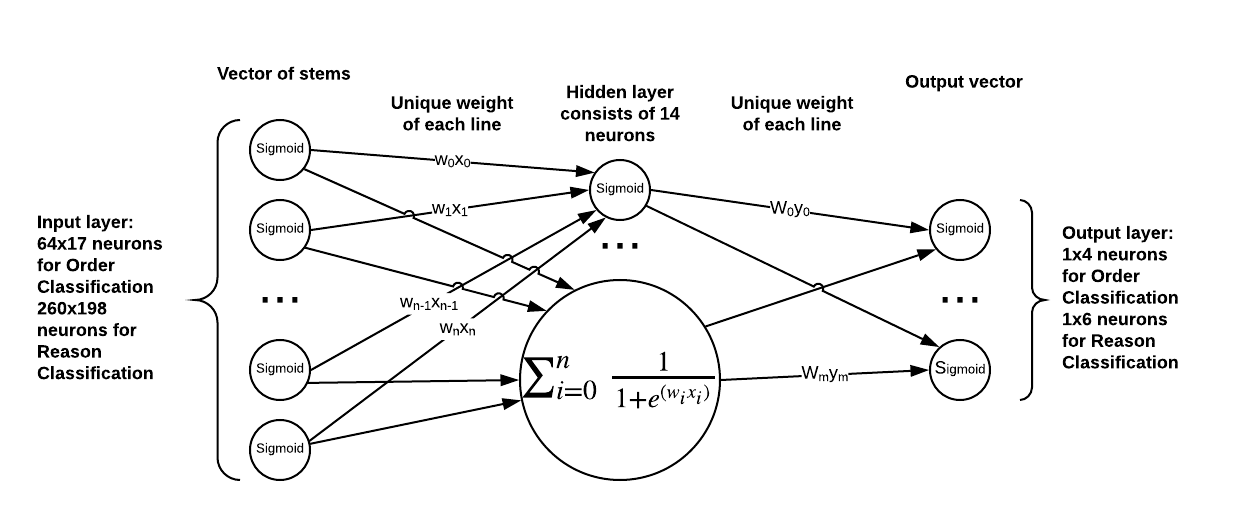
\includegraphics[width=\textwidth]{ANN.png}
        \caption[]{Classification Neural Network Topology}
    \end{figure}
    Topology of the Artificial Neural Network consists of Input, Output and Hidden layers.\\
    \em Input layer \em consist of input neurons that are binomial representation of the unique stemmed words inside the text that is already cleaned from punctuation and meaningless words like articles.
    While morphological variants are different word forms, they represent same concept.
    In text categorization and other similar tasks it is desirable to combine these morphological variants of the same word into one canonical form and represent it like vector that is called stemmed version.\\
    \em Output layer \em gives vector of possibilities that the text is inside of classes.
    The most possible class is the classification answer of the neural network.\\
    \em Hidden layer \em is the regression function of FNN, or layer between input and output layers.
    FNN applies a sequence of linear functions to the data.
    These functions are sigmoid linear transformation of the previous layer.
    As a result, it followed by a squashing nonlinearity.
    The most efficient number of hidden layer neurons (14) was found by calculation of the delta that was found by
    1000 iterations of Backpropogation training algorithm.\\
    In the next example user typed that he wants to change device status because he needs to finish a project about flu.
    Classifier says that it is 99.9\% about work, and a little bit (0.05\%) about heath issue, because his project about flu.\\
    \begin{example}
        User input is: I need to finish my project about flu\\
        System classified it as: 'Work': 0.999, 'Health': 0.0566
    \end{example}
    The Backpropagation learning rule based on supervised learning was used \cite{14}.
    In order to train neural network, a set of training documents and a specification of the pre-defined categories the
    documents belong to are required.
    Training and testing sets were created specially for this experiment.\\
    Rule-Based Reasoner receives data about the user`s order and compares it with rules in the Database and actual status of the devices.
    Core of the Rule-Based Reasoner is the set of if-else rules.
    Firstly, RBR checks the status of the device and compares it with order.
    Secondly, it checks is there conflict between user command and rule.
    If there is a conflict it executes Case-Based Reasoner (CBR).\\
    CBR is an artificial intelligence approach to determine a similarity amongst a set of cases.
    CBR is the foundation of the many intelligent systems.
    This method indexes cases from history of the system usage and retrieves best similar case by measurement of distance between the input case and past cases.
    The result of finding best match is stored inside the cases database to update the cases database and adapt old solution to the new variables and environment.
    CBR is based on a suggestion that the similar cases have similar solution \cite{7}.\\
    Most of the CBR systems uses k-nearest neighbour algorithm.
    The accuracy of this classification algorithm seriously depends on the metrics or system of measurement used to compute distances between different cases.
    The nearest neighbour algorithm determines the similarity or dissimilarity of a new case with the case base and follows a cyclical process of Retrieve-Reuse-Revise-Retain.
    In our case inputs to the system are in different systems of measurements.
    Cases in the system are build on preferences and priority of users of the system.
    Both two variables have different basis.
    As a result, standard Euclidean Distance cannot be used as a distance measurement algorithm.\\
    It was proposed to use Mahalanobis distance that is the global linear transformation tool of the input spaces of the cases from different classes separated by a large margins.
    Using of Mahalanobis distance significantly increases kNN accuracy \cite{17}.\\
    \section{Sequences}
    %
    Sequences inside the system are mentioned in this chapter.
    Sequence diagram of the system can be found in figure below.
    It shows two main scenarios inside the system.\\
    \begin{figure}
        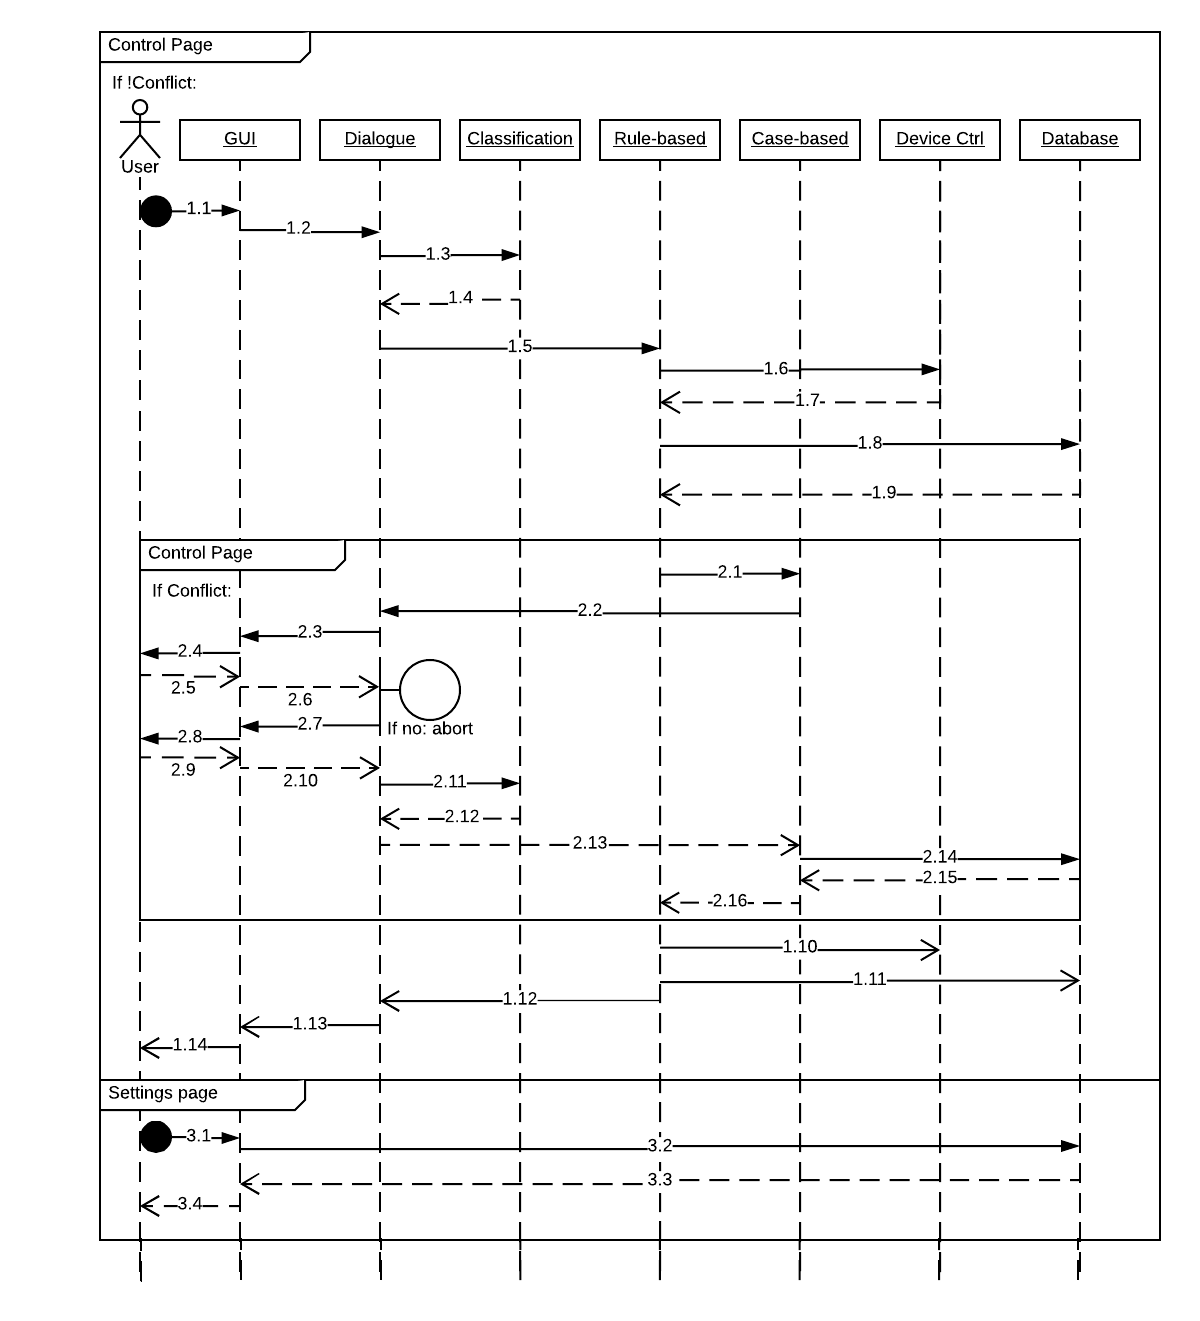
\includegraphics[width=0.7\textwidth]{UML.png}
        \caption[]{UML Sequence diagram of the system}
    \end{figure}
    First of all, the user sends command to the system (1.1) that is analysed by Dialogue Component (1.2) via Classification ANN (1.3, 1.4).
    Next, system sends classified order to the RBR (1.5) and checks it`s context (1.6 - 1.9).
    If there is no conflict, it changes device status (1.10, 1.11) and answers to the user (1.12 - 1.14).
    Else, it executes Conflict Resolution Scenario by Case-Based Reasoner (2.1).\\
    Next, it informs the user about conflict (2.2 - 2.4) and wait command.
    If the user cancels command (2.5, 2.6), it aborts Conflict Resolution loop.
    Else, the system asks for argumentation (2.7, 2.8) from user (2.9, 2.10) and classifies it (2.11, 2.12).
    After collection of data (2.13) CBR reads old cases (2.14, 2.15) and makes a decision (2.16).\\
    \section{Results and Validation}
    %
    In order to perform randomized double
    blinded experiment, we developed scenario creating sub-module.
    Firstly, it creates random scenario for tester by choosing
    conflicting device and reasons for tester by using crypto-secure randomise function based on operation system inner
    clocks.
    Secondly, it provides such instructions to testers where he or she was
    asked to provide commands in their own words.
    As a result, scenarios were hidden from us and testers till
    the beginning of the experiment.\\
    In addition, thirteen testers were asked to fill evaluation form.
    In the evaluation form testers were asked to answers questions with quantitative form, where 0 is very badly and 4 is very good, about Speech recognition,
    classification, conflict resolution, total idea, interface design, interaction with VA and user friendliness.
    Furthermore, they were provided with additional text box under each question to justify their answers.\\
    The majority of the responses were positive \footnote{83 of 91 quantitative answers are positive, 5 neutral and 3 negative.}
    and the average of the all answers are higher the "Good" level (3 and more) except "Conflict Resolution" question, which
    has 2.9 average value with 1.2 standard deviation amount.\\
    The question about conflict resolution quality was the most complicated for the system, because it has two negative answers.
    Firstly, there was disagreement about priorities policy of the system and the general view of the user.
    The tester did not agree that the adult has higher priority with entertainment issue versus younger with work issue.
    The second case was unique and new to the CBR, and it did not managed to give appropriate output.
    Analysis of the system logs and simulation of the case gave us better understanding of the system fault.
    As a result, there is a list of possible cause effects and ways to solve them.
    Firstly, lack of training data can be solved by creating more training cases and store them into Databases.
    Second, changing the input matrix formulation might be solution.\\
    \section{Conclusion}
    This paper presents Virtual Assistant in the multiple user Smart Home environment.
    The Virtual Assistant was created
    to manage and monitor Smart Home environment by dialogue based interaction with users.
    Different machine learning
    algorithms and cloud technologies were implemented to meet project objectives.
    The main focus of the research was to
    develop adaptive context aware conflict resolution system based on Case-Based Reasoner.
    The validation tests feedback is positive.\\
    The future direction of the work is to implement context-aware system that analyzes user behaviour and reports it as
    a case to the database of Case-Based Reasoner.
    In order to change paradigm from technology centered perspective to human centered perspective,
    it is significant to introduce behaviour adapting sub-system \cite{2}.
    In addition, it is recommended to implement machine learning algorithms to measure distances between cases to
    increase accuracy of the Case-Based Reasoner.\\
    All the materials and sources of the system can be found in the GitHub repository of the project \footnote{https://github.com/BiggyBaron/VirtualAssistant}.
    \begin{thebibliography}{1}
        \bibitem {1}
        Alirezaie, M., Renoux, J., Köckemann, U., Kristoffersson, A., Karlsson, L., Blomqvist, E., Tsiftes, N., Voigt, T., Loutfi, A.: An Ontology-based Context-aware System for Smart Homes: E-care@home. Sensors. 17, 1586 (2017).

        \bibitem {2}
        Aztiria, A., Augusto, J., Basagoiti, R., Izaguirre, A., Cook, D.: Learning Frequent Behaviors of the Users in Intelligent Environments. IEEE Transactions on Systems, Man, and Cybernetics: Systems. 43, 1265-1278 (2013).

        \bibitem {3}
        Fleury, A., Vacher, M., Noury, N.: SVM-Based Multimodal Classification of Activities of Daily Living in Health Smart Homes: Sensors, Algorithms, and First Experimental Results. IEEE Transactions on Information Technology in Biomedicine. 14, 274-283 (2010).

        \bibitem {5}
        Hadj, R., Hamon, C., Chollet, S., Vega, G., Lalanda, P.: Context-based conflict management in pervasive platforms. 2017 IEEE International Conference on Pervasive Computing and Communications Workshops (PerCom Workshops). (2017).

        \bibitem {6}
        Kabir, M., Hoque, M., Seo, H., Yang, S.: Machine Learning Based Adaptive Context-Aware System for Smart Home Environment, https://pdfs.semanticscholar.org/8cf5/fe5062727744f5429bb34d9c0bd24f439ee6.pdf.

        \bibitem {7}
        Khan, N., Alegre, U., Kramer, D., Augusto, J.: Is ‘Context-Aware Reasoning = Case-Based Reasoning’?. Modeling and Using Context. 418-431 (2017).

        \bibitem {8}
        Mayer, S., Inhelder, N., Verborgh, R., Van de Walle, R., Mattern, F.: Configuration of smart environments made simple: Combining visual modeling with semantic metadata and reasoning. 2014 International Conference on the Internet of Things (IOT). (2014).

        \bibitem {9}
        Nurgaliyev, K., Mauro, D., Khan, N., Augusto, J.: Improved Multi-user Interaction in a Smart Environment Through a Preference-Based Conflict Resolution Virtual Assistant. 2017 International Conference on Intelligent Environments (IE). (2017).

        \bibitem {10}
        Oguego, C., Augusto, J., Muñ`oz, A., Springett, M.: A survey on managing users’ preferences in ambient intelligence. Universal Access in the Information Society. (2017).

        \bibitem {11}
        Oguego, C., Augusto, J., Muñoz, A., Springett, M.: Using argumentation to manage users’ preferences. Future Generation Computer Systems. 81, 235-243 (2018).

        \bibitem {12}
        Ospan, B.: Simulation of a Simple Bio-Mimetic Robot with Neuromorphic Control System and Optimization Based on the Genetic Algorithm. International Journal of Innovations in Engineering and Technology. 8, 59-65 (2017).
        \bibitem {13}
        Portet, F., Vacher, M., Golanski, C., Roux, C., Meillon, B.: Design and evaluation of a smart home voice interface for the elderly: acceptability and objection aspects. Personal and Ubiquitous Computing. 17, 127-144 (2011).

        \bibitem {14}
        Ramasundaram, S., Victor, S.: Text Categorization by Backpropagation Network, http://www.ijcaonline.org/archives/volume8/number6/1217-1754.

        \bibitem {15}
        Reichherzer, T., Satterfield, S., Belitsos, J., Chudzynski, J., Watson, L.: An Agent-Based Architecture for Sensor Data Collection and Reasoning in Smart Home Environments for Independent Living. Advances in Artificial Intelligence. 15-20 (2016).

        \bibitem {17}
        Weinberger, K., Lawrence, S.: Distance Metric Learning for Large Margin Nearest Neighbor Classification. Journal of Machine Learning Research. 10, 207-244 (2009).

    \end{thebibliography}

\end{document}